\section{{\color{red}Results - Scale Testing}}
\label{ResultsScaleTesting}
%
The dataset contains several zero-answers, which can happen when subjects doesn't answer on a scale. To exclude some of the zero-points that occured because of a non-answered scale two criterias is stated: 1) If all scale ratings presented on one of the pages are zero, it's probably because subjects skipped a page and 2) If there is a tendency for high ratings on a scale and a zero-answer seems unlikely, it's probably a missing answer.\\

\noindent
The different ratings on the scales in the second test are visualised on \autoref{fig:Boxplot}.
%
\begin{figure}[H]
\centering
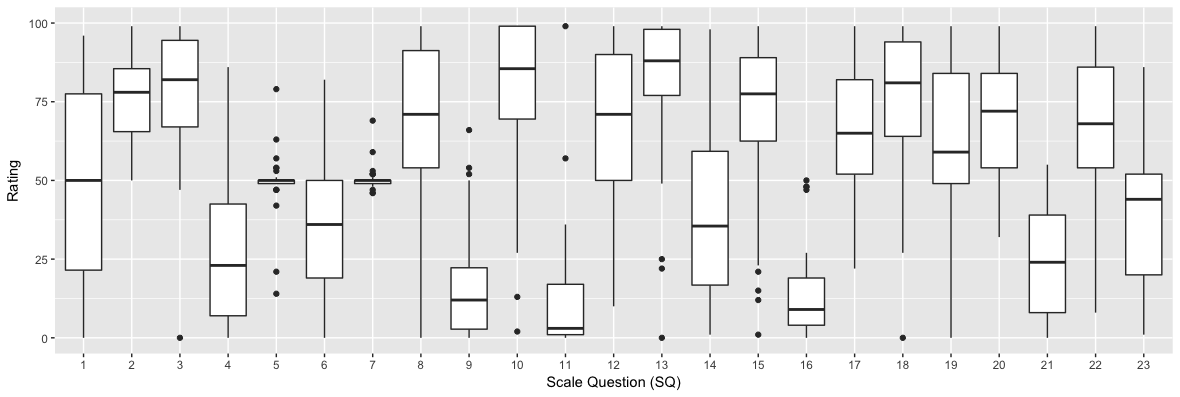
\includegraphics[width = 0.49\textwidth]{Figure/Boksplot0er}
\setlength\abovecaptionskip{-1.2\baselineskip} 
\caption{Boxplot showing the 24 variables. The boxplot contains a median, the box ranging from 25-75 \% and the whiskers from 0-25 \% and 25-100 \%, respectively.}
\label{fig:Boxplot}
\end{figure}
\noindent
%
From the boxplot it is seen that......\\
 
\noindent
SQ5 and SQ7 is centered around the mid point, which can reltate to the label (fine) being to wide a label. Subjects are answering around the midpoint regardless of the height of the robot or how close to them it stops. The two variables are seen to have an impact on the experience interacting with robots in the reviewed litterature, so they might be expressed even though they are not included as scales.

When looking at gender differences SQ4 and SQ21 seems to reveal a difference. Women rates SQ4 and SQ21 twice as high as men, which means that they experience the robot's movements more calm but also more intrusive.
%
\begin{figure}[H]
	\centering
	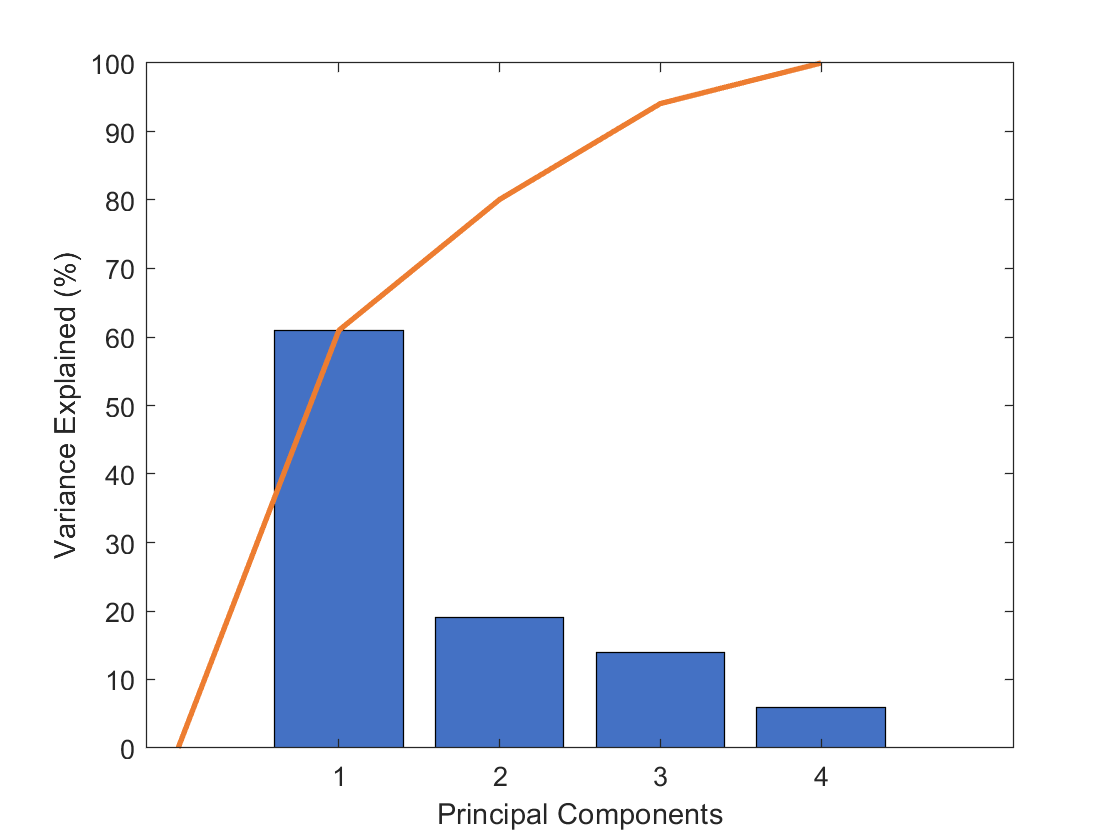
\includegraphics[width = 0.49\textwidth]{Figure/Scree.png}
	\setlength\abovecaptionskip{-1.2\baselineskip} 
	\caption{Scree plot showing the connection between the number of Principal Components and Variance Explained [\%].}
	\label{fig:Scree}
\end{figure}
\noindent
%
Conducting a PCA on the data results in the screeplot on \autoref{fig:Scree}. It shows that when using 7 dimension only 80 \% of the variance is explained, which is why PCA relating to different groups as the robot's height, distance and direction is conducted. \autoref{fig:biplot} shows the biplot relating to the robot's height. Similar biplots are made for direction and distance. 
%
\begin{figure}[H]
	\centering
	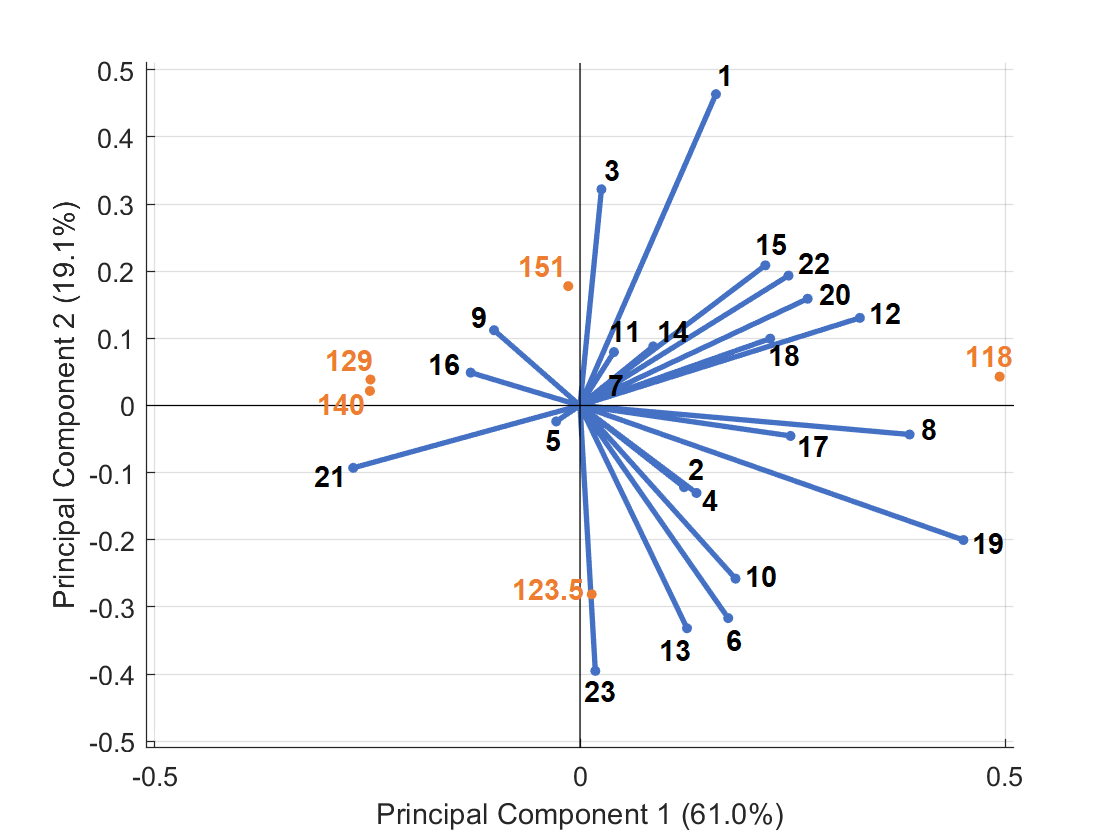
\includegraphics[width = 0.49\textwidth]{Figure/RHeight-Biplot.png}
	\setlength\abovecaptionskip{-1.2\baselineskip} 
	\caption{Biplot showing how the different variables contributes to components and which variables correlates. The black numbers relates the the SQ and the red to the different heights.}
	\label{fig:biplot}
\end{figure}
\noindent
%
%
\begin{figure}[H]
	\centering
	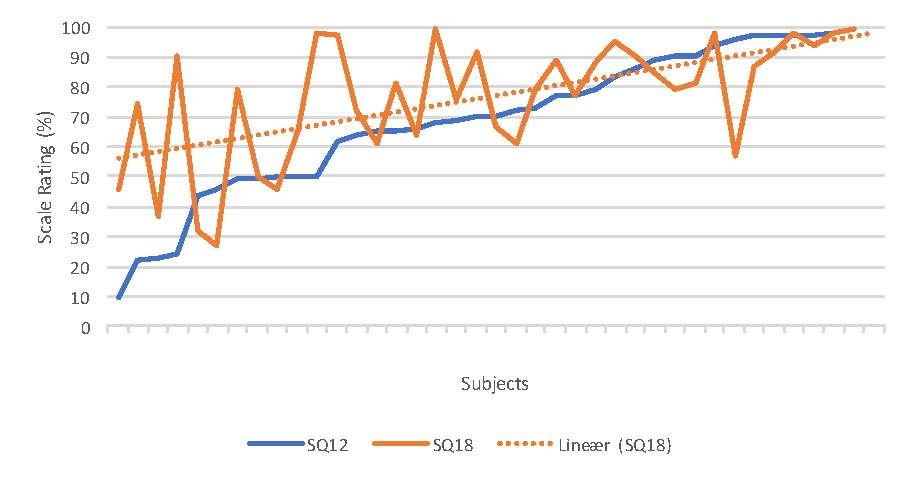
\includegraphics[width = 0.49\textwidth]{Figure/SQ12+SQ18}
	\setlength\abovecaptionskip{-1.2\baselineskip} 
	\caption{NEW.}
	\label{fig:SQ12+SQ18}
\end{figure}
\noindent
%
%
\begin{figure}[H]
	\centering
	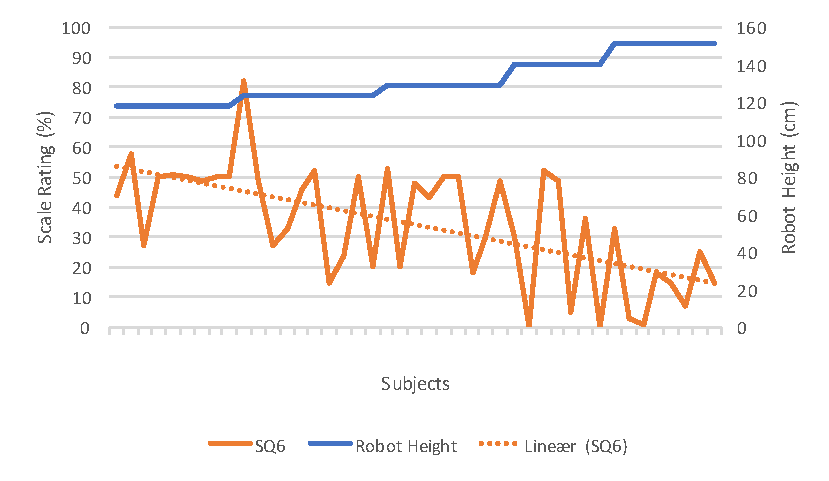
\includegraphics[width = 0.49\textwidth]{Figure/HeightSQ6}
	\setlength\abovecaptionskip{-1.2\baselineskip} 
	\caption{NEW.}
	\label{fig:HeightSQ6}
\end{figure}
\noindent
%


{\color{red} Her præsenteres resultater fra analysen af vores resultater fra anden test. Hvor resultaterne er fra Principal component analysis}
%\blankline
%
Det der tænkes at resultater skal indeholde: 
\begin{itemize}
	\item Forklare at det er eksplorativ databehandling/studie
	\item Fortælle om overordnede PCA - som ikke forklarer særlig meget af variansen.
	\item Præsenter PCA højde - hvad korrelere og er der noget der er redundant.
	\item Præsenter PCA indgangsvinkel - hvad korrelere og er der noget der er redundant.
	\item Præsenter PCA afstand - hvad korrelere og er der noget der er redundant.
\end{itemize}